\chapter{相关工作}

为了更好地设计适用于日常健康场景下的面诊系统,本章将介绍当前比较流行的基于面诊技术的面诊系统设计,最后简单介绍本文的研究方法。

\section{面诊系统}

面诊系统是基于面诊算法为用户提供面诊功能的一套系统。
目前已经有不少研究将面诊技术落地,下面将主要介绍代表性的几类,同时简单概括其特点以及不足之处。

\begin{figure}[h]
    \centering
    \subfigure[面诊仪]{
        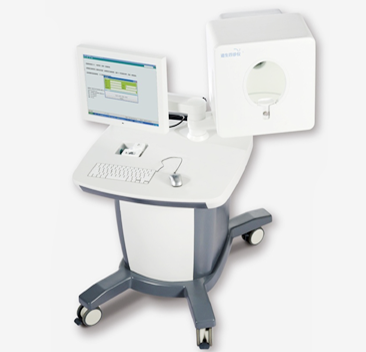
\includegraphics[height=6cm]{images/mzy.png}
    }
    \subfigure[云中医智能镜]{
        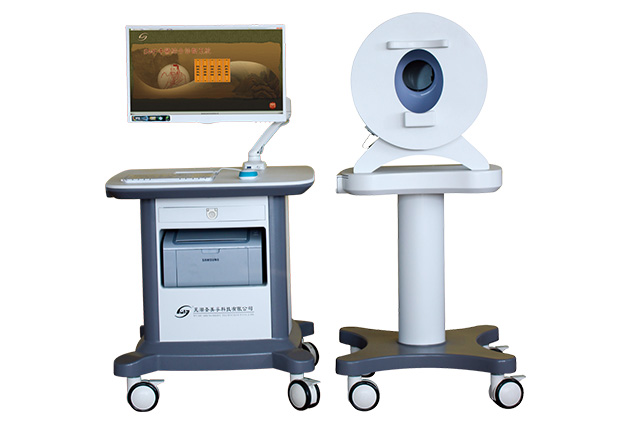
\includegraphics[height=6cm]{images/SMF.jpg}
    }
    \caption{面诊仪}
    \label{fig:med}
\end{figure}

\subsection{面诊仪}
目前面诊技术最主要的应用场景是医疗环境中的各类面诊仪。面诊仪如舌面象仪可作为初步信息采集工具得到患者的面色,舌象等信息,而面色自动识别分析系统则能得出初步的诊断结果,然后由医生根据这些信息得到最终结果\cite{崔骥2018人工智能背景下中医诊疗技术的应用与展望}。
面诊仪如道生面诊仪\cite{邸丹2016手持式舌象仪的研制}是目前某些医院用来采集面部信息的设备, 芜湖圣美孚科技有限公司\footnote{http://www.smfkj.com/}也有一款舌面诊一体化设备,
这类系统可以实现面部图像采集以及面部特征提取,如面色、唇色、舌苔、舌象等,为诊断提供依据。

但面诊仪主要是医疗环境中使用,不适合日常场景下:这类面诊系统因为依赖特有的设备,操作比较复杂,需要在中医医师的指导下,进行舌相面色诊断信息采集,最终结果需要中医医师进行判断。
此外,当前技术发展非常迅速,当新的面诊算法出现时,面诊仪没有合适的算法更新和添加机制,设备迭代成本较大。

\subsection{云中医}

\begin{figure}
    \centering
    \subfigure[云中医智能镜]{
        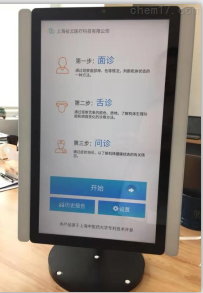
\includegraphics[width=4.5cm]{images/yzy.png}
    }
    \subfigure[云中医诊断机器人]{
        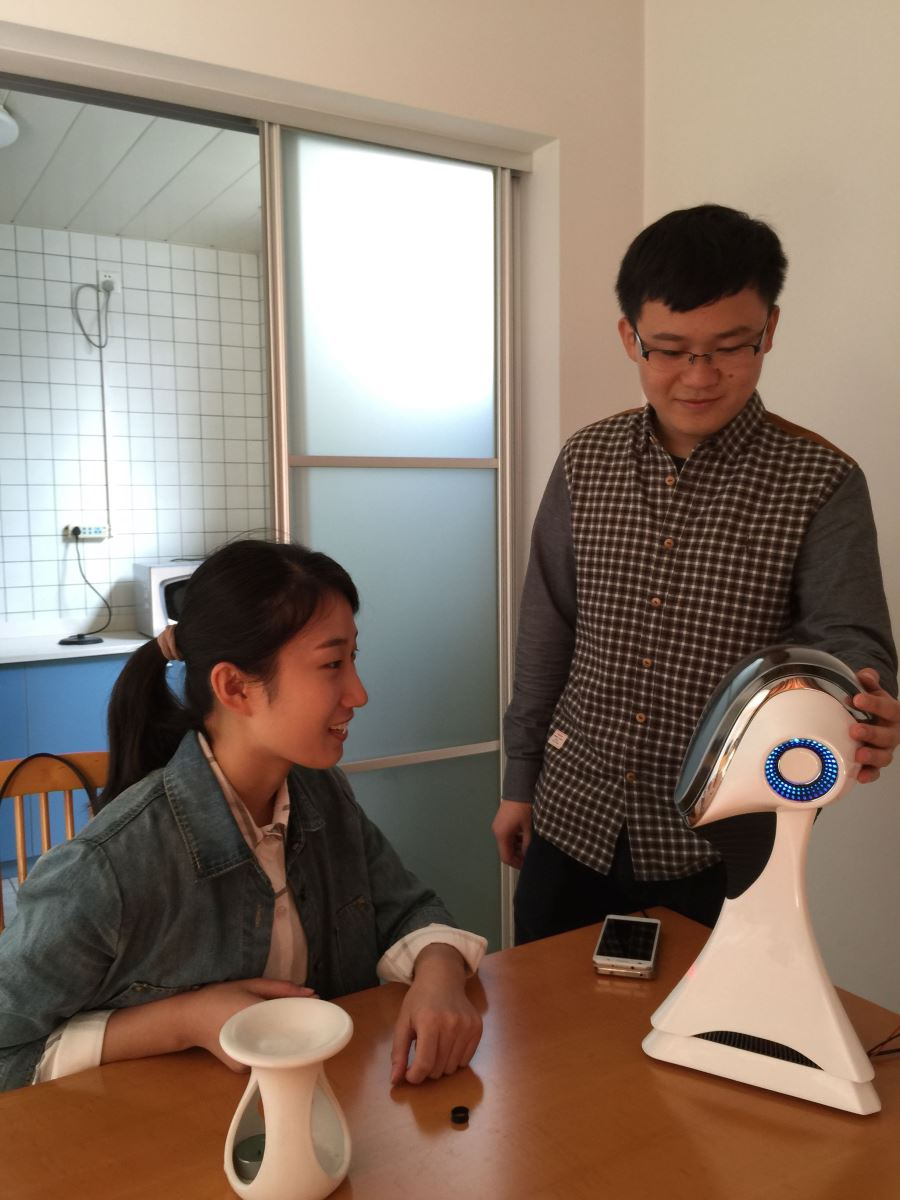
\includegraphics[width=4.5cm]{images/med_robot.jpg}
    }
    \subfigure[云中医应用]{
        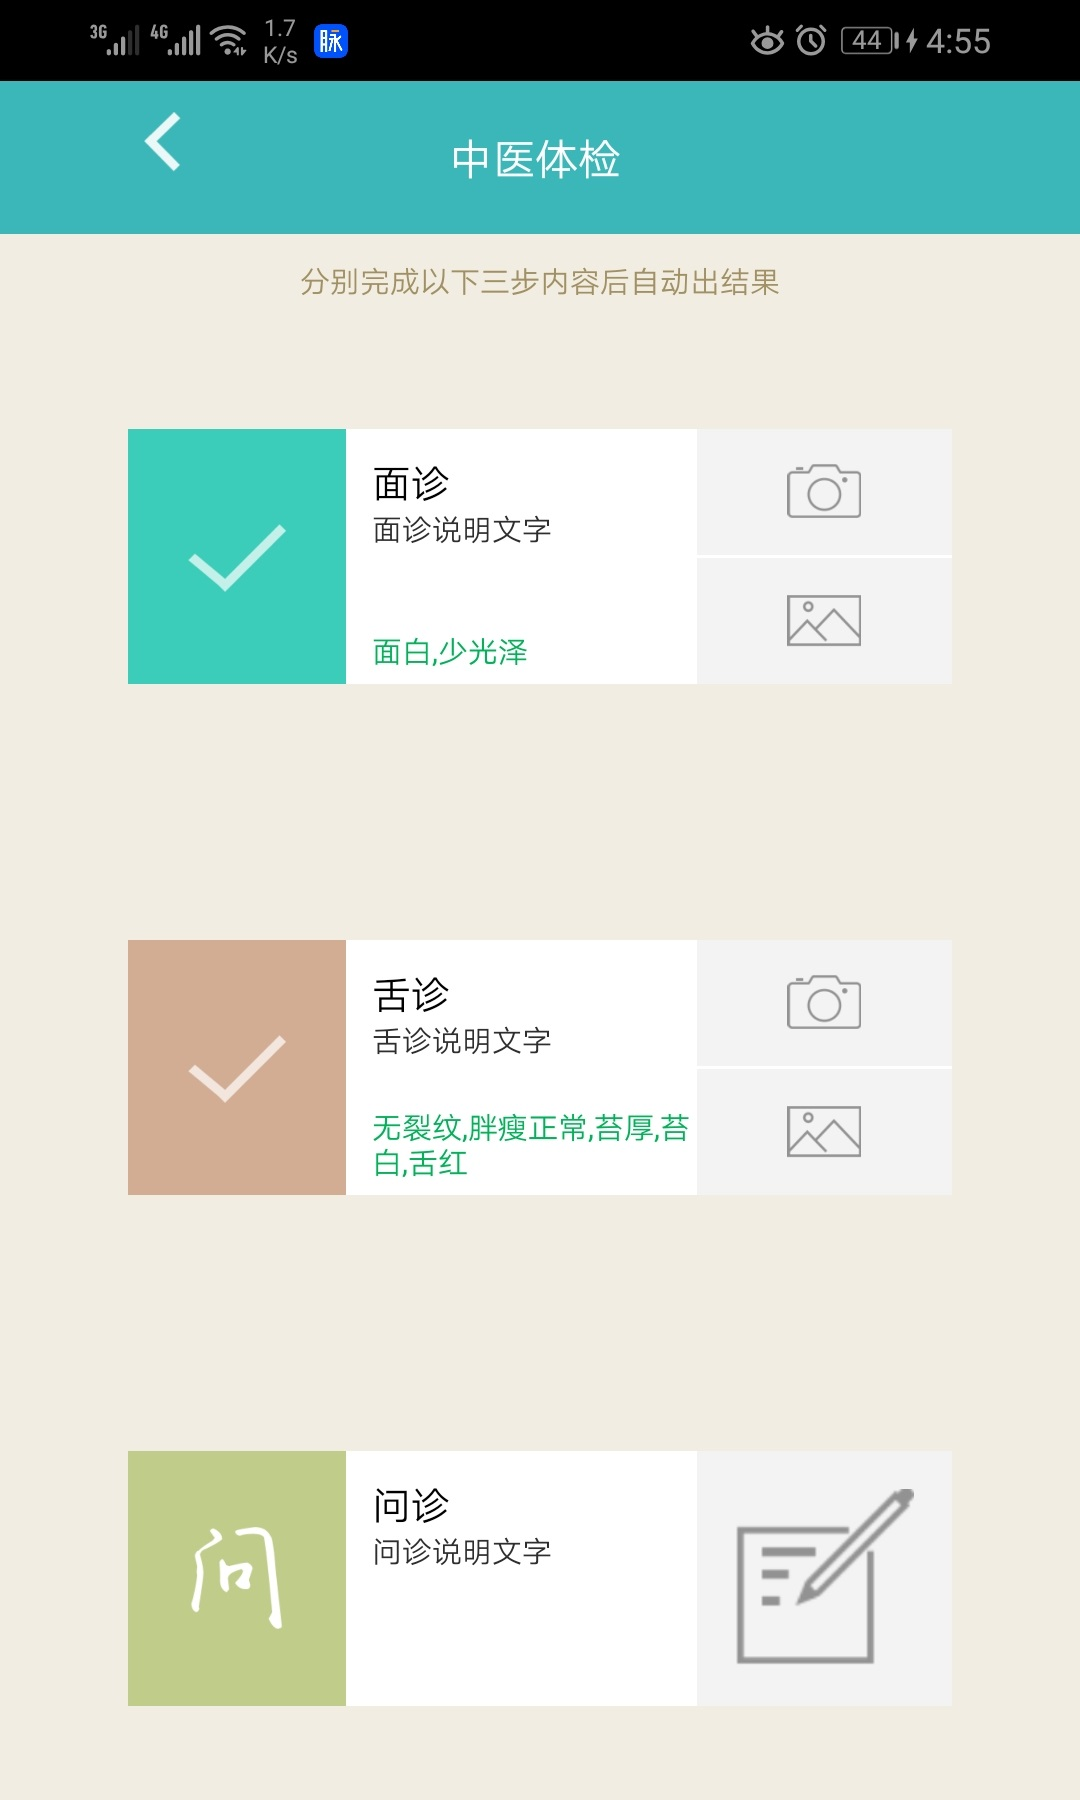
\includegraphics[width=4.5cm]{images/main1.jpg}
    }
    \caption{云中医系列产品}
    \label{fig:cloudmed}
\end{figure}

云中医是复旦大学计算机学院张文强老师和上海中医药大学合作开发的一款面诊应用,旨在为用户提供一个方便的自我诊断和健康管理平台,目前主要应用场景是各大社区、诊所给用户做健康参考。该应用以中医面诊、舌诊、问诊理论为指导,在手机上模拟实现了诊断的过程:用户需要依次对自己的面部和舌头进行拍照,回答一些与自己健康状况相关的问题,最终会收到一份完整的健康报告和一些健康建议。

\begin{figure}[h]
    \centering
    \subfigure[主界面]{
        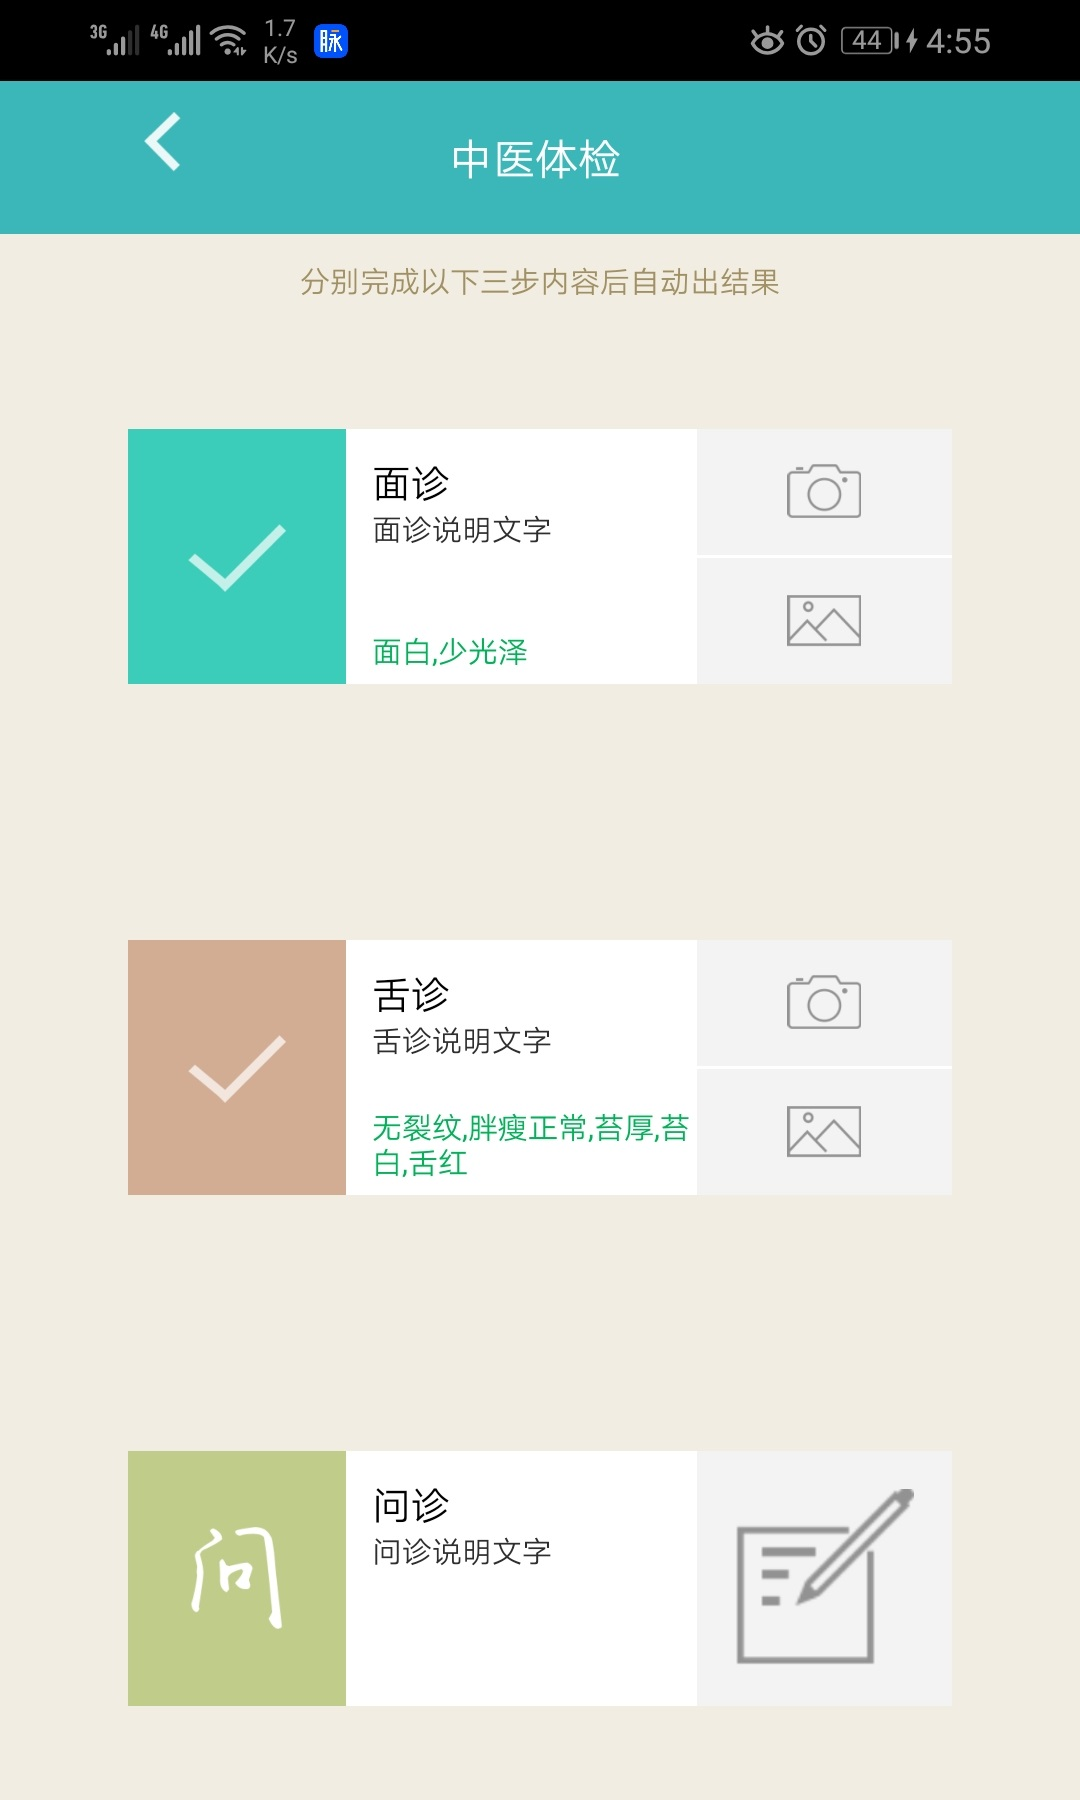
\includegraphics[width=4.5cm]{images/main1.jpg}
    }
    \subfigure[问诊]{
        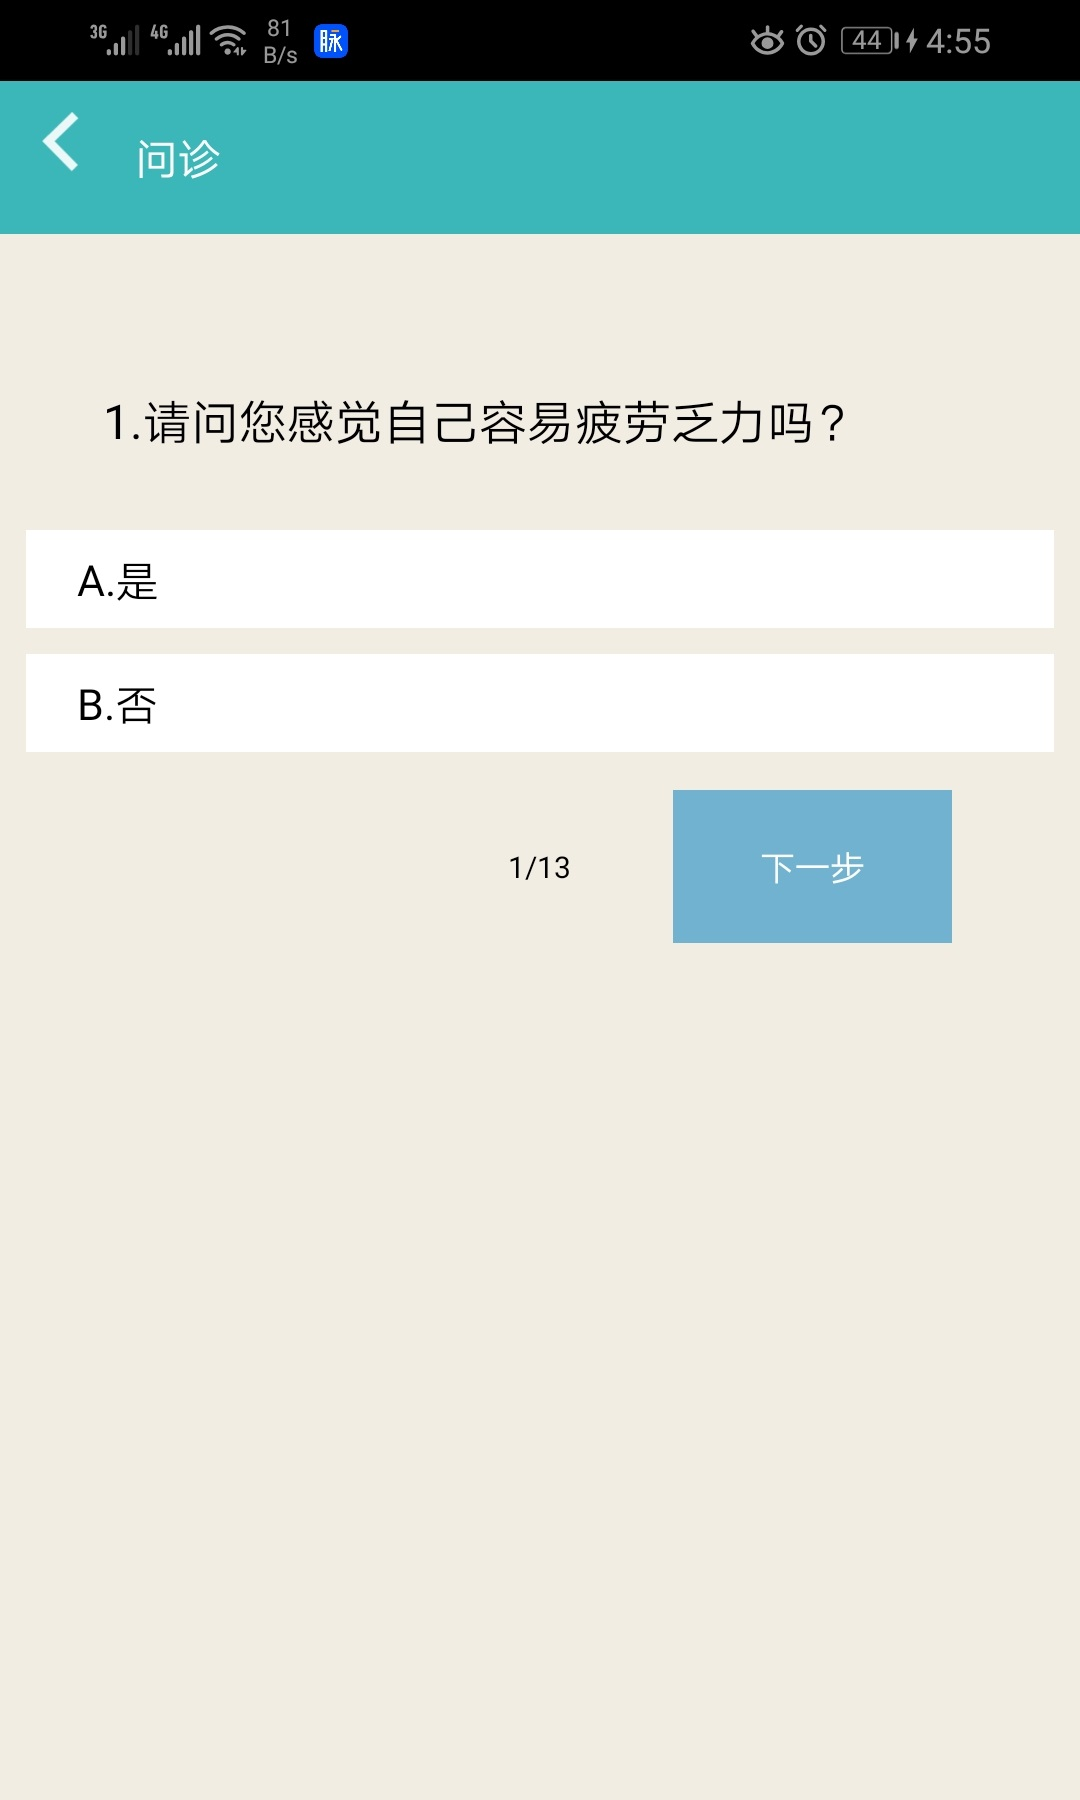
\includegraphics[width=4.5cm]{images/main2.jpg}
    }
    \subfigure[健康报告]{
        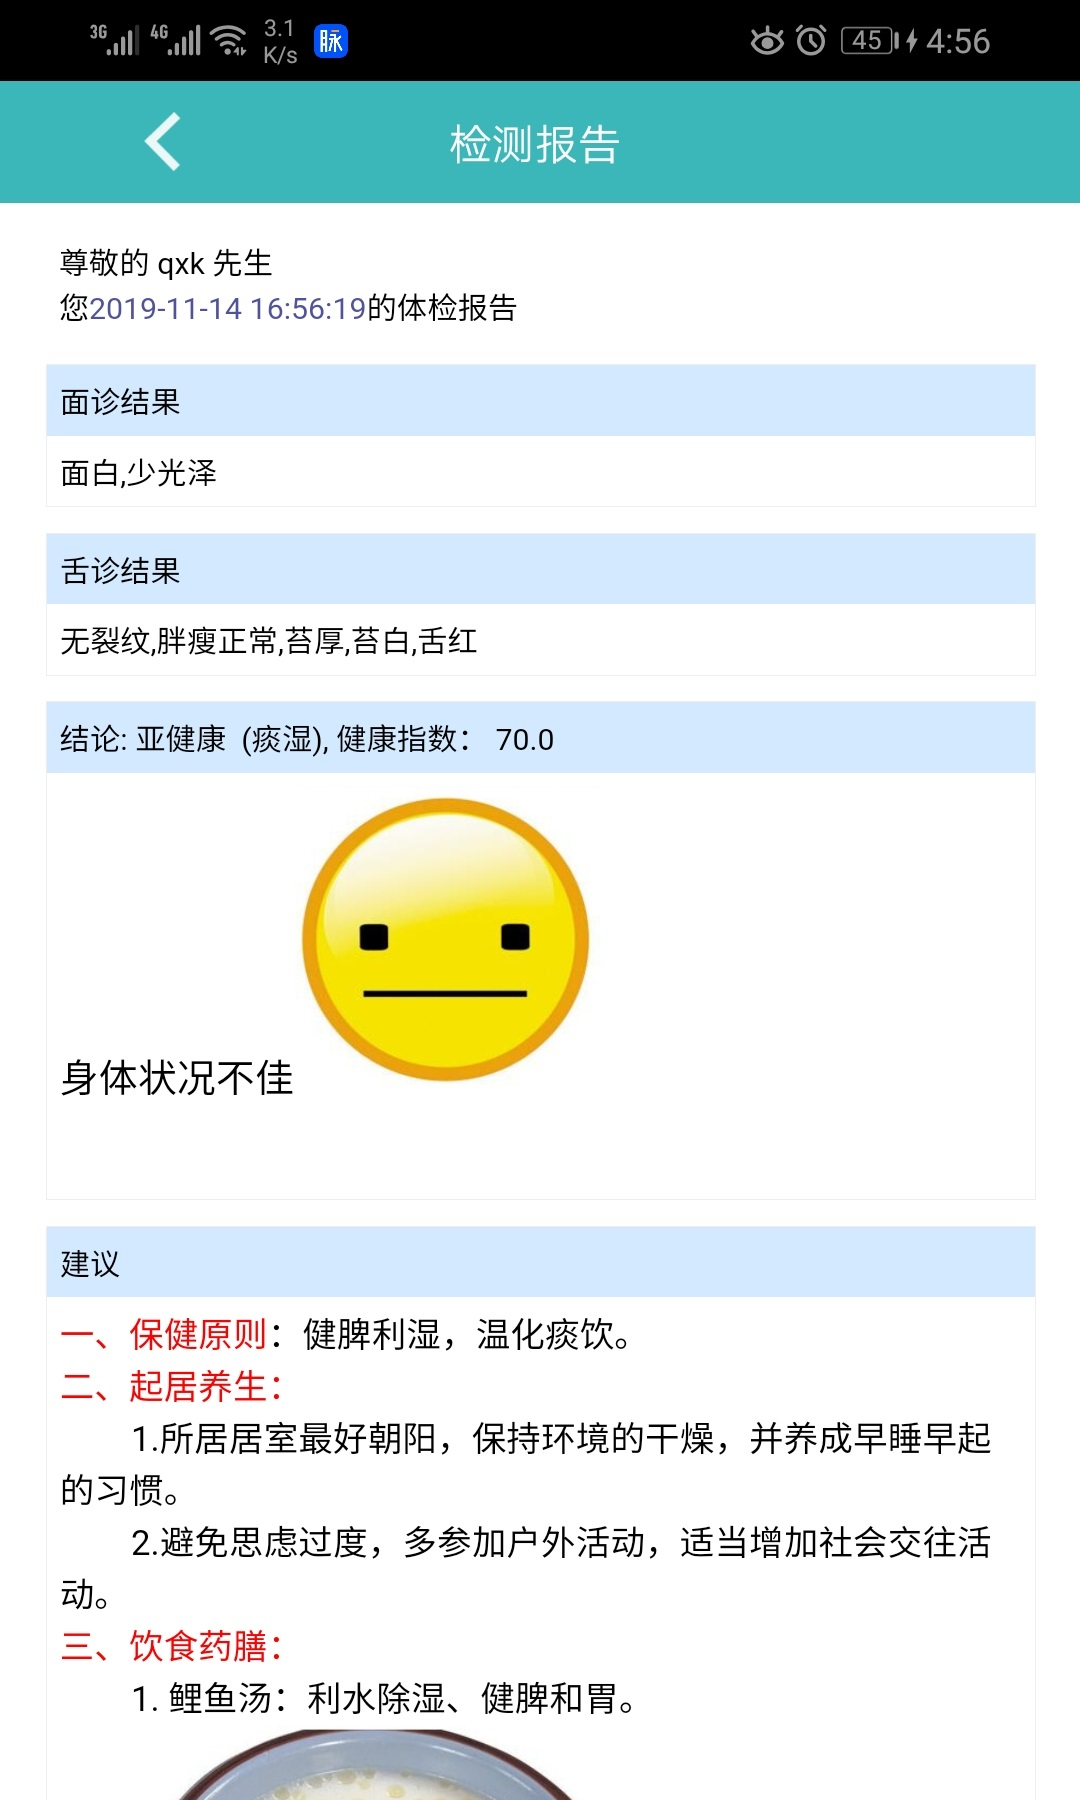
\includegraphics[width=4.5cm]{images/main3.jpg}
    }
    \caption{云中医主要界面}
    \label{fig:main}
\end{figure}

云中医应用的主要界面及使用流程如图 \ref{fig:main}所示:用户进入诊断页面之后,会看到三个区域:面诊、舌诊、问诊。面诊和舌诊通过拍照或者上传图片完成,问诊是通过依次回答13个问题来完成。依次完成面诊、舌诊、问诊后,系统会给出用户的体质和健康分数,并且给出对应的健康建议。

云中医的系统设计对设备要求比较灵活,在移动设备、机器人平台上都有对应的产品,其中包括云中医诊断机器人\footnote{http://www.sohu.com/a/135358060\_205169/},云中医智能镜\cite{李雪2016},云中医应用\cite{钱鹏基于云中医的健康监测方法及系统}等,但是遗憾的是,云中医虽然功能比较齐全,但是其主要应用场景是社区和诊所等公共环境,缺乏日常健康环境下的用户研究和交互研究。
同时,云中医的算法为端到端模式,把相关的算法都内嵌在一个模型中。
对于用户来说整个系统就是一个黑盒,后续研究中本文也发现黑盒模式不利于提高用户对系统的理解和信赖程度。

\subsection{SEMEOTICONS}

\begin{figure}[h]
    \centering
    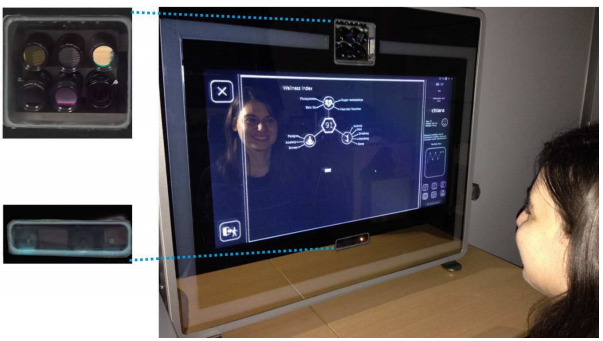
\includegraphics[width=12cm]{images/mirror.png}
    \caption{SEMEOTICONS}
    \label{fig:seme}
\end{figure}
如图 \ref{fig:seme} 所示,Yasmina Andreu-Cabedo等 \cite{andreu2015mirror}则开发了SEMEOTICONS系统。
SEMEOTICONS是一款放在家庭室内环境的镜子,通过摄像头和传感器采集面部信息和体温,监测与心血管疾病相关的疲劳、压力和焦虑等特征, 让用户能够监测自己的健康情况,并根据量身定制的健康指南来改善用户的生活方式。该系统由室内的硬件设备和远程服务器一起完成健康监测的功能,室内设备负责采集数据,远程服务器负责处理数据分析结果。
在生活中照镜子本来就是每个人的日常行为,该研究将读脸技术和健康管理结合起来,并且将应用场景拓展到了日常环境。
他们后续还进行了一次用户体验调研,调研结果表明\cite{coppini2017user} 他们的原型系统的设计被大多数用户所接受: 虽然测试过程非常耗时,大多数参与研究中的志愿者仍然很愿意完成并按计划进行实验,部分志愿者考虑了系统给出的健康指南,甚至因此改变了自己的生活方式。

总的来说,该系统通过将诊断和日常的照镜子的行为结合起来,可以很方便与用户的日常生活融合起来,同时在服务器端也可以方便的实现算法模型的适配和更新。
但是该系统固定在房间的某个位置使用的方式不够便携,同时该系统需要一系列的传感器设备,不仅增加了硬件的成本,部署起来也相对麻烦,而且只能在室内使用。


\section{本文研究方法}

% 定性研究, 强调context的重要性,以人为中心,重视用户的体验。
人机交互(Human-Computer Interaction)的研究以人为中心,涵盖计算机科学、社会学、心理学等学科,重视技术如何更好地为人服务\cite{lazar2017research}。
在探索以人为中心的相关交互设计、系统设计方面,人机交互研究也有相关的方法论以及数据获取方法\cite{lazar2017research}。

本小节将简单介绍本文的研究方法以及数据获取方法。

% 研究方法

\subsection{技术探针}

% 为什么要用技术探针
通常,典型的人机交互研究中研究系统设计是访问用户的家庭,然后设计并实现一个系统,让用户评价。
在日常场景下,这种设计方法缺点比较明显\cite{Hutchinson2003Technology}:

\begin{itemize}
    \item 没有激发用户的思考,可能无法反映用户的实际需求和掩盖在家庭内部之间"好玩”的设计。
    \item 在设计和实现系统过程中,没有提供真实的长期使用场景,用户缺乏参与性。  
\end{itemize}


% 介绍什么是技术探针
为了避免上述的问题,Hutchinson等\cite{Hutchinson2003Technology}提出了一种利用快速开发出来的、功能并不完善的原型系统,让用户在实际使用原型系统的过程中,鼓励用户大声表达自己异想天开的想法,在草稿上画出自己心中的系统,参与设计过程的研究方法。

基于技术探针的方法经常被用来为日常使用的健康技术的设计提供信息。例如通过技术探针的设计方法,Papi等人\cite{papi2015knee}利用可穿戴式膝关节原型,探索了在家庭环境下如何设计用于骨关节炎患者的康复工具;同样,Singh等人\cite{singh2017supporting}通过1-2周的用户研究,利用技术探针,研究了如何设计慢性疼痛患者使用的日常可穿戴设备。

% 数据采集方法
\subsubsection{研究数据获取}
在计算机领域,常见的用户数据获取是通过大量统计数据,如大批量结构化的问卷、用户行为日志等,然后在分析过程中,通过提取自变量、因变量做变量的相关性分析得到最终的结论。

在人机交互研究中,通常采用获取数据的方法是通过资料分析、案例分析、直接观察、用户访谈等方式获取研究数据。其中,深度访谈是交互研究领域中收集数据最常用的一种方式,通过开放式、半结构化的面对面访谈,能够深度了解调查者内心的客观想法,避免研究者的主观判断。该方法在心理学与社会学领域被广泛应用,能够发掘出用户更细节的需求和想法。
同时,该方法对数据量的是要求不高,在连续访谈得到的结果比较稳定后就可以停止访谈。

本文使用两者相结合的方式获取研究数据,首先通过分析日志和问卷,得到大致的结论,然后通过面对面深度访谈发掘更深层次的原因,得到最终的结论。

% 技术探针, 文化探针 等

\section{本章小结}
本章主要介绍了当前主要的面诊系统设计已经各自的特点和不足,同时为了方便读者理解,本章还介绍了本文的研究方法和数据获取方法。

